\chapter{2 GW Network Representation in RSCAD}

\section{MMCs and HVAC cables in Draft module}
\begin{figure}[H]
\centering
%\hspace*{-0.2cm}
    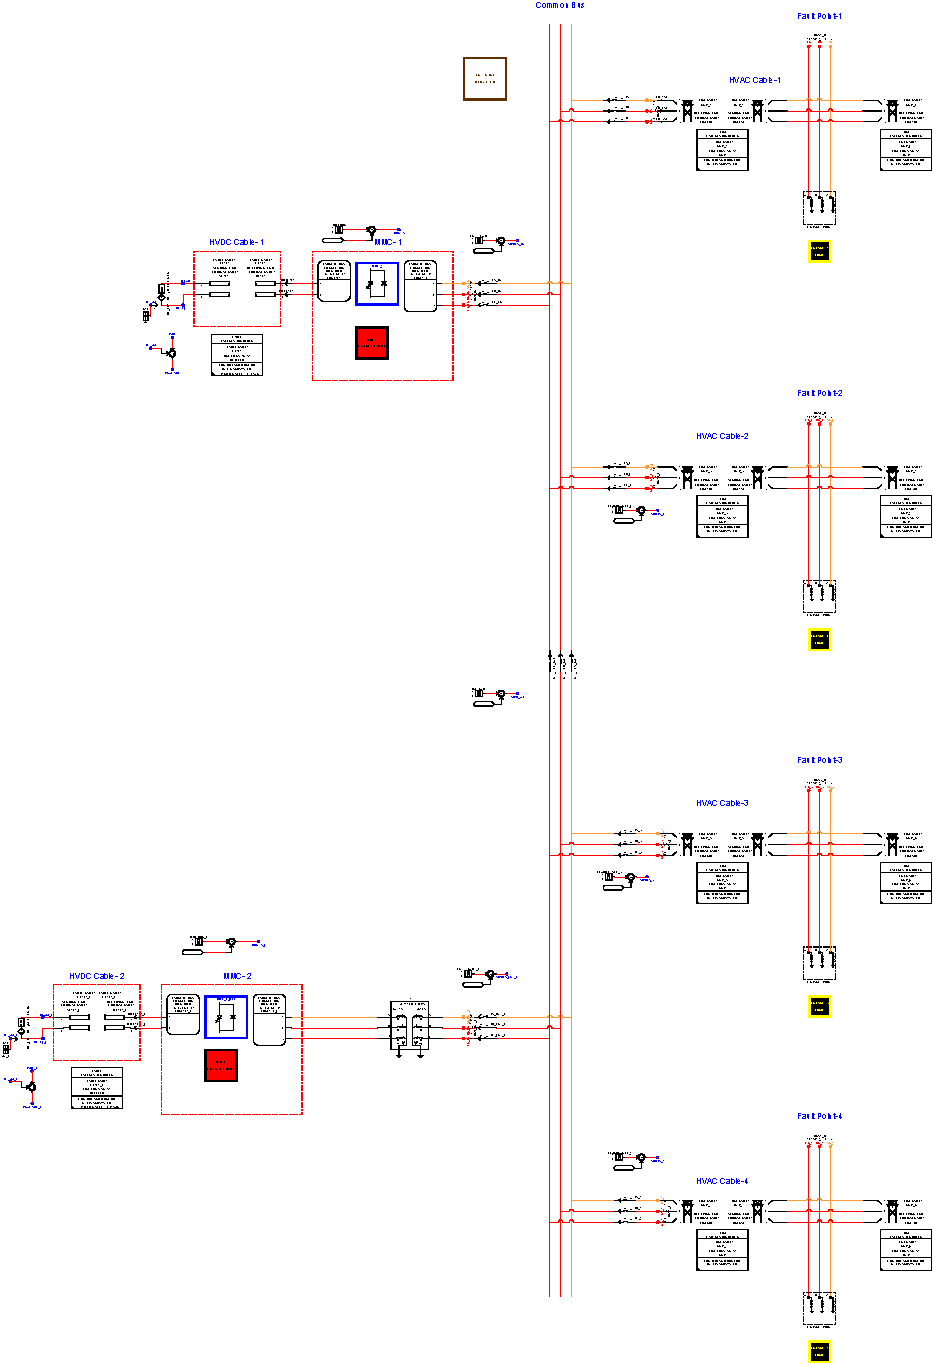
\includegraphics[height = 16cm,width = 10.5cm]{Diagrams/Appendix_C/MMC_2_RSCAD_Rep.pdf}
    \caption{Subsystem-1: 66 kV HVAC cables connected to offshore MMC stations in Draft module in RSCAD}
    \label{fig:MMC_2_RSCAD_Rep}
\end{figure}

\section{OWFs in Draft module}

\begin{figure}[H]
\centering
%\hspace*{-0.2cm}
    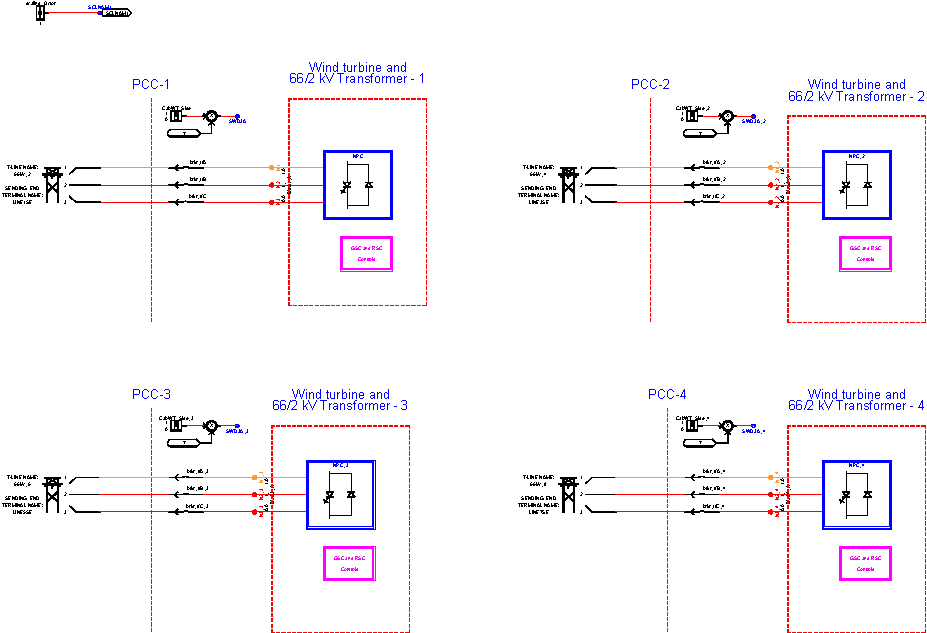
\includegraphics[height = 11cm,width = \textwidth]{Diagrams/Appendix_C/MMC_2_RSCAD_Rep_2.pdf}
    \caption{Subsystem-2: OWFs connected to HVAC cables in Draft module in RSCAD}
    \label{fig:MMC_2_RSCAD_Rep_2}
\end{figure}

\subsection{Modification in Outer Loop Control}\label{modific_outer_loop}
In order to simplify the system, the active power loop output variable which is the active power reference (idref2) is made to be controlled by the user using a slider (ID\_ref\_control) in Runtime file directly as shown in Figure \ref{fig:Idref_control}. This allows the user to control the amount of active power flowing through the \gls{MMC}-2 bus. The 'ID\_ref\_control' value is varied from 0 to a maximum of 0.4. There is no flow of power in \gls{MMC}-2 when 'ID\_ref\_control' = 0. The maximum power flow is achieved when 'ID\_ref\_control' = 0.4. 

The RMS current (I\_rms) is calculated at the breaker (CB-1a) and is compared with the maximum current (I\_phase\_max) which is 10\% above the phase current as given in Equation \ref{i_phase_max_eq}. When 'I\_rms' current exceeds 'I\_phase\_max', 'idref2' is set to zero for that duration. Once, 'I\_rms' becomes less than 'I\_phase\_max', the control is given back to 'ID\_ref\_control' slider in Runtime module, as shown in Figure \ref{fig:Idref_control}. This allows power to flow in \gls{MMC}-2 after the breaker CB-1a has been operated.

\begin{equation}
    I_{phase} = \frac{S_{single\_phase}}{V_{LN}}
\end{equation}

\begin{equation}\label{i_phase_max_eq}
    I_{phase\_max} = 1.1 * I_{phase}
\end{equation}

\begin{figure}[H]
\centering
%\hspace*{-1.2cm}
    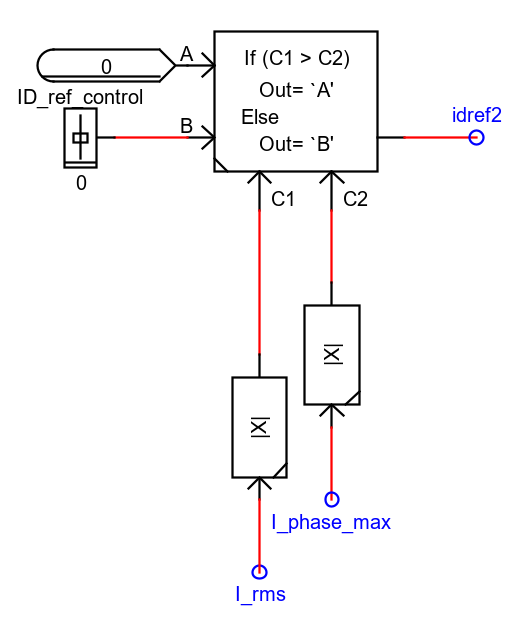
\includegraphics[height = 6cm,width = 5.5cm]{Diagrams/Chapter_4/Idref_control.PNG}
    \caption{Idref2 control logic}
    \label{fig:Idref_control}
\end{figure}

\section{Steps for operation of the model in Runtime module}

Scaling factor is set to 10 before simulation.
ID\_ref\_control is also set to 0 before starting the simulation.

\subsection{Energization of the network}\label{energ_appendix}

\begin{itemize}
    \item Compile the Draft file "WT4\_MMC2\_Draft.dft" and ensure there are no errors.
    \item Open the Runtime file "WT4\_MMC2\_Draft.sib".
    \item Switch on the 'MMCBRK' switch to charge the \gls{MMC} bus.
    
    \begin{figure}[H]
\centering
%\hspace*{-1.2cm}
    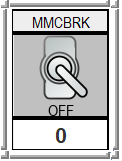
\includegraphics[height = 2cm,width = 2cm]{Diagrams/Appendix_C/MMCBRK.PNG}
    \caption{MMCBRK switch}
    \label{fig:MMCBRK}
\end{figure}
    
    \item Switch on the 'MMCBRK\_2' switch to connect \gls{MMC}-2 to the network.
    
    \begin{figure}[H]
\centering
%\hspace*{-1.2cm}
    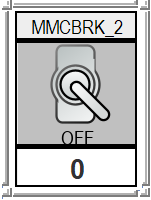
\includegraphics[height = 2cm,width = 2cm]{Diagrams/Appendix_C/MMCBRK_2.PNG}
    \caption{MMCBRK\_2 switch}
    \label{fig:MMCBRK_2}
\end{figure}
    
    \item Switch on the 'CabMMC\_Side' breaker switch to charge Cable-1. Then switch on 'CabWT\_Side' breaker switch to connect \gls{OWF}-1 to the network.
    
      \begin{figure}[H]
\centering
%\hspace*{-1.2cm}
    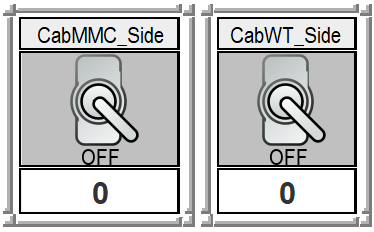
\includegraphics[height = 2cm,width = 3.5cm]{Diagrams/Appendix_C/Cab_1.PNG}
    \caption{CabMMC\_Side and CabWT\_Side switches}
    \label{fig:Cab_1}
\end{figure}  
    
    \item Switch on the 'CabMMC\_Side\_2' breaker switch to charge Cable-2. Then switch on 'CabWT\_Side\_2' breaker switch to connect \gls{OWF}-2 to the network.
 
     \begin{figure}[H]
\centering
%\hspace*{-1.2cm}
    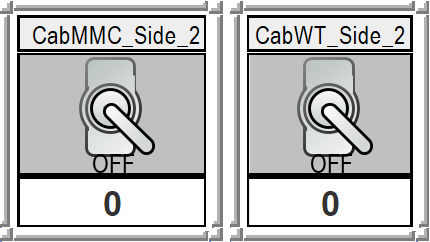
\includegraphics[height = 2cm,width = 3.5cm]{Diagrams/Appendix_C/Cab_2.PNG}
    \caption{CabMMC\_Side\_2 and CabWT\_Side\_2 switches}
    \label{fig:Cab_2}
\end{figure}
    
    \item Switch on the 'CabMMC\_Side\_3' breaker switch to charge Cable-3. Then switch on 'CabWT\_Side\_3' breaker switch to connect \gls{OWF}-3 to the network.
    
        \begin{figure}[H]
\centering
%\hspace*{-1.2cm}
    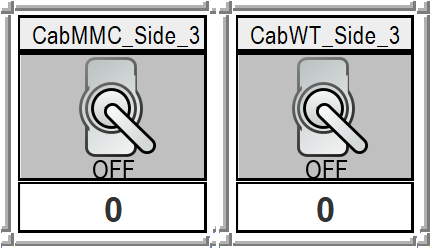
\includegraphics[height = 2cm,width = 3.5cm]{Diagrams/Appendix_C/Cab_3.PNG}
    \caption{CabMMC\_Side\_3 and CabWT\_Side\_3 switches}
    \label{fig:Cab_3}
\end{figure}

    \item Switch on the 'CabMMC\_Side\_4' breaker switch to charge Cable-4. Then switch on 'CabWT\_Side\_4' breaker switch to connect \gls{OWF}-4 to the network.
    
        \begin{figure}[H]
\centering
%\hspace*{-1.2cm}
    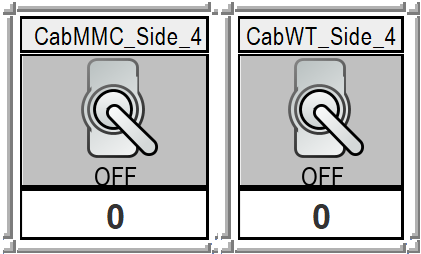
\includegraphics[height = 2cm,width = 3.5cm]{Diagrams/Appendix_C/Cab_4.PNG}
    \caption{CabMMC\_Side\_4 and CabWT\_Side\_4 switches}
    \label{fig:Cab_4}
\end{figure}

\end{itemize}
After the final step, nearly 200 MW active power flows through \gls{MMC}-1 and there is no power flow in \gls{MMC}-2.


\subsection{Full generation from OWFs and power flow in MMC-1 and MMC-2}\label{full_gen_appendix}
    \begin{itemize}
        \item Increase scaling\_factor from 10 to 40.
        \item Change ID\_ref\_control from 0 to 0.2.
        \item Increase scaling\_factor from 40 to 60.
        \item Change ID\_ref\_control from 0.2 to 0.3.
        \item Increase scaling\_factor from 60 to 80.
        \item Change ID\_ref\_control from 0.3 to 0.38.
        \item Increase scaling\_factor from 80 to 90.
        \item Change ID\_ref\_control from 0.38 to 0.4.
        \item Finally, increase scaling\_factor from 90 to 92.
    \end{itemize} 

A total of nearly 2 GW power flows in the network after the above steps. 1 GW through \gls{MMC}-1 and 1 GW through \gls{MMC}-2.


 \begin{table}[H]
 \centering
\begin{tabular}{|c|c|}
\hline
\textbf{ID\_ref\_control} & \textbf{Power through MMC-2} \\ \hline
0                    & 0 MW                         \\ \hline
0.2                  & 475 MW                       \\ \hline
0.4                  & 950 MW                       \\ \hline
\end{tabular}
\caption{Power flow control in MMC-2}
\label{tab:Power_flow_control_in_MMC-2}
\end{table}

\subsection{Disconnection of set of OWF}
\gls{OWF}-2 is chosen for this thesis. 
\begin{itemize}
    \item Open the breaker switch 'CabMMC\_Side\_2' to disconnect \gls{OWF}-2.
    \item The above test can also be performed on other \gls{OWF}s as well by opening 'CabMMC\_Side' for \gls{OWF}-1, 'CabMMC\_Side\_3' for \gls{OWF}-3 and 'CabMMC\_Side\_4' for \gls{OWF}-4 respectively.
\end{itemize}

\subsection{Three-phase line to ground fault in the middle of a HVAC cable}
The control logic in Figure \ref{fig:Idref_control} and the breaker logic in Section \ref{fig:Fault_logic} is modelled for \gls{HVAC} cable-1 for this work. 

First, the steps \ref{energ_appendix} and \ref{full_gen_appendix} must be performed to achieved 2 GW power transmission.

\begin{itemize}
    \item Switch on the 'Active' switch  to change control of circuit breaker CB-1a from 'CabMMC\_Side' switch to the logic explained in Section \ref{Fault logic and cb}. The network still operates in steady state in this condition.
    \item Apply the fault by clicking the 'LG\_FLT8' button (red in colour).
\end{itemize}

\begin{figure}[H]
\centering
%\hspace*{-1.2cm}
    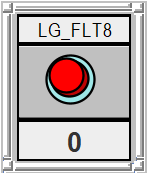
\includegraphics[height = 2cm,width = 1.75cm]{Diagrams/Appendix_C/Fault_button.PNG}
    \caption{Fault button}
    \label{fig:Fault_button}
\end{figure}

\section{Additional graphs}
\subsection{Disconnection of OWF-2}

\begin{figure}[H]
%\centering
%\hspace*{-1.2cm}
    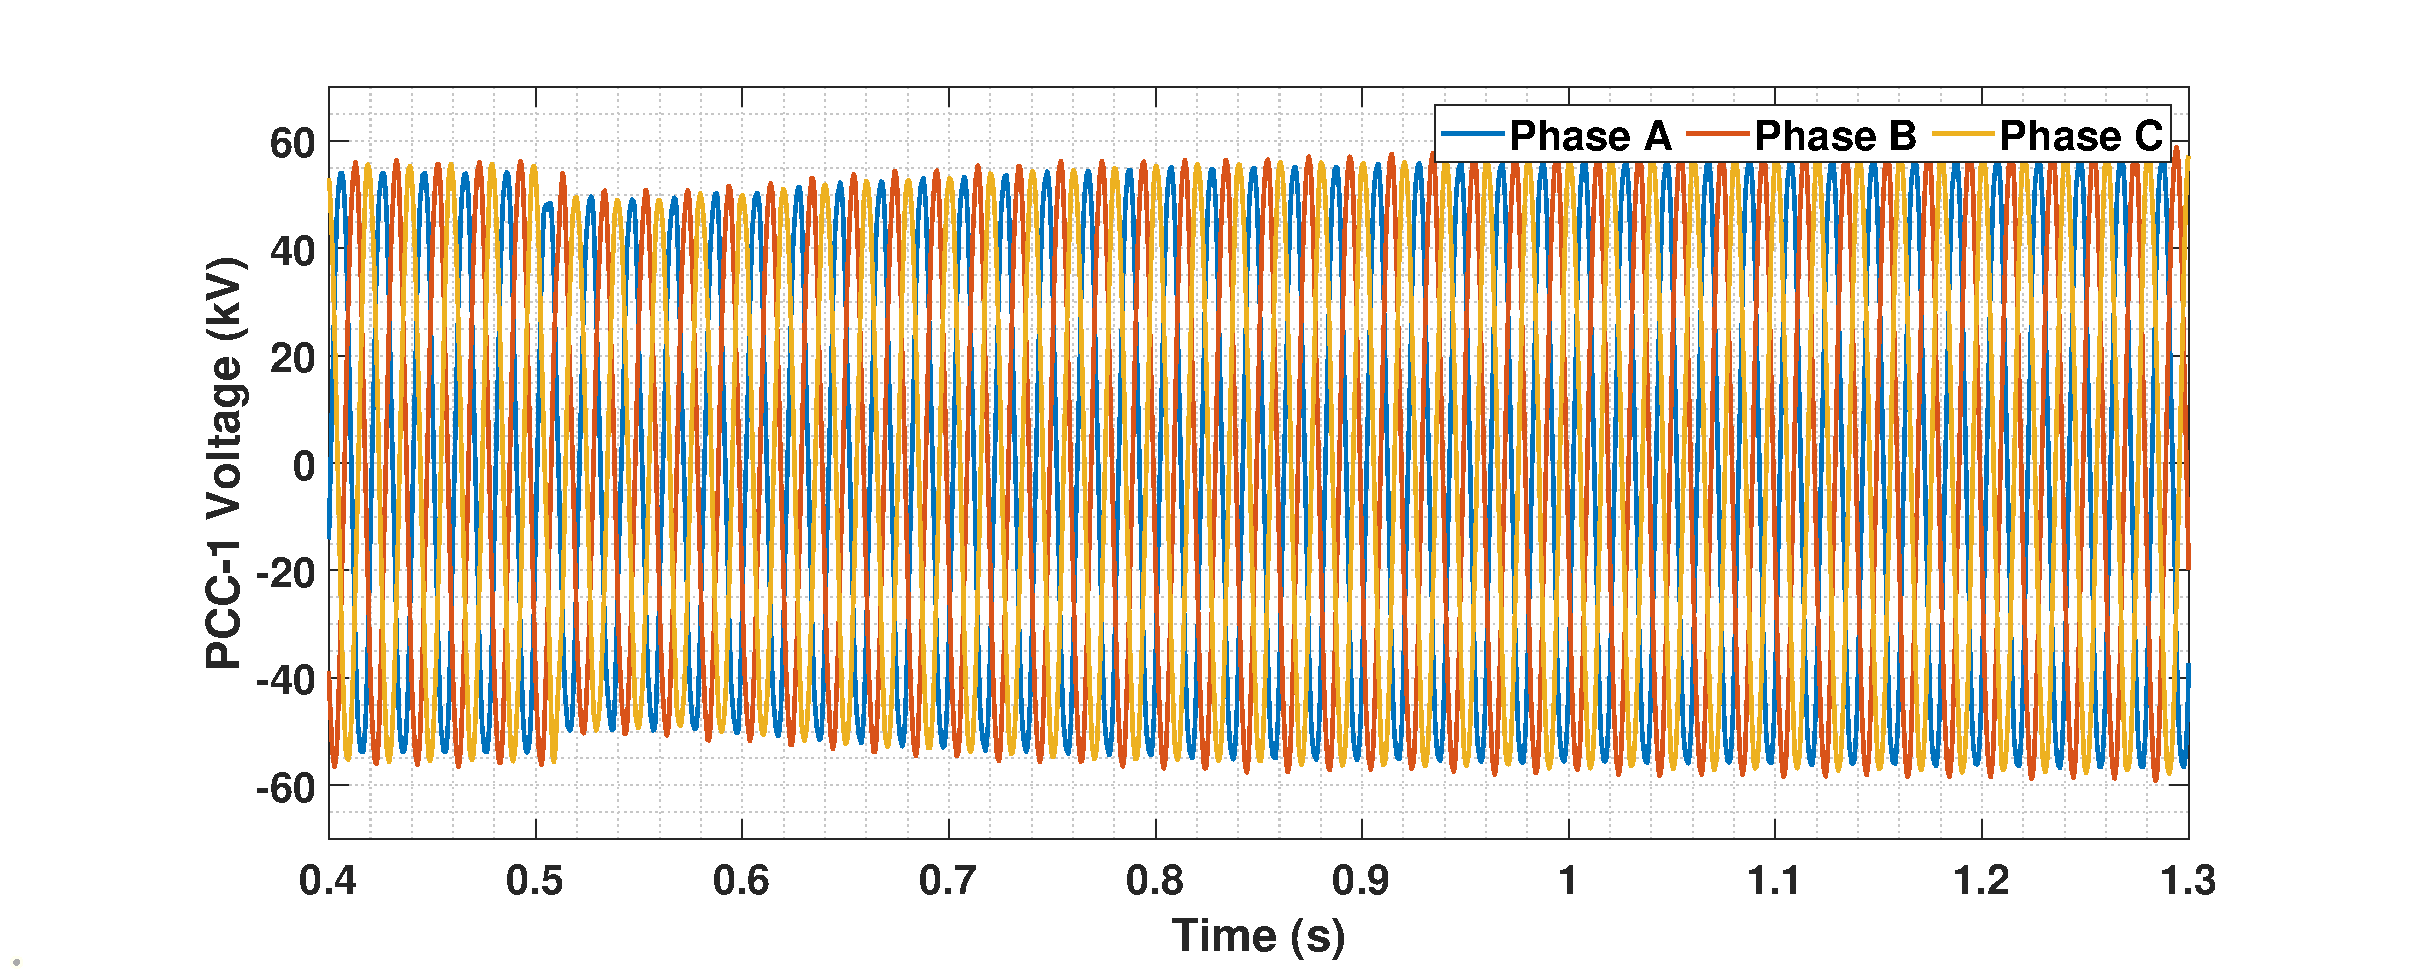
\includegraphics[height = 7cm,width = \textwidth]{Diagrams/Appendix_C/VABC_WT1_WT2off.eps}
    \caption{Voltages at PCC-1 upon OWF-2 disconnection event}
    \label{VABC_WT1_WT2off}
\end{figure}

\begin{figure}[H]
%\centering
%\hspace*{-1.2cm}
    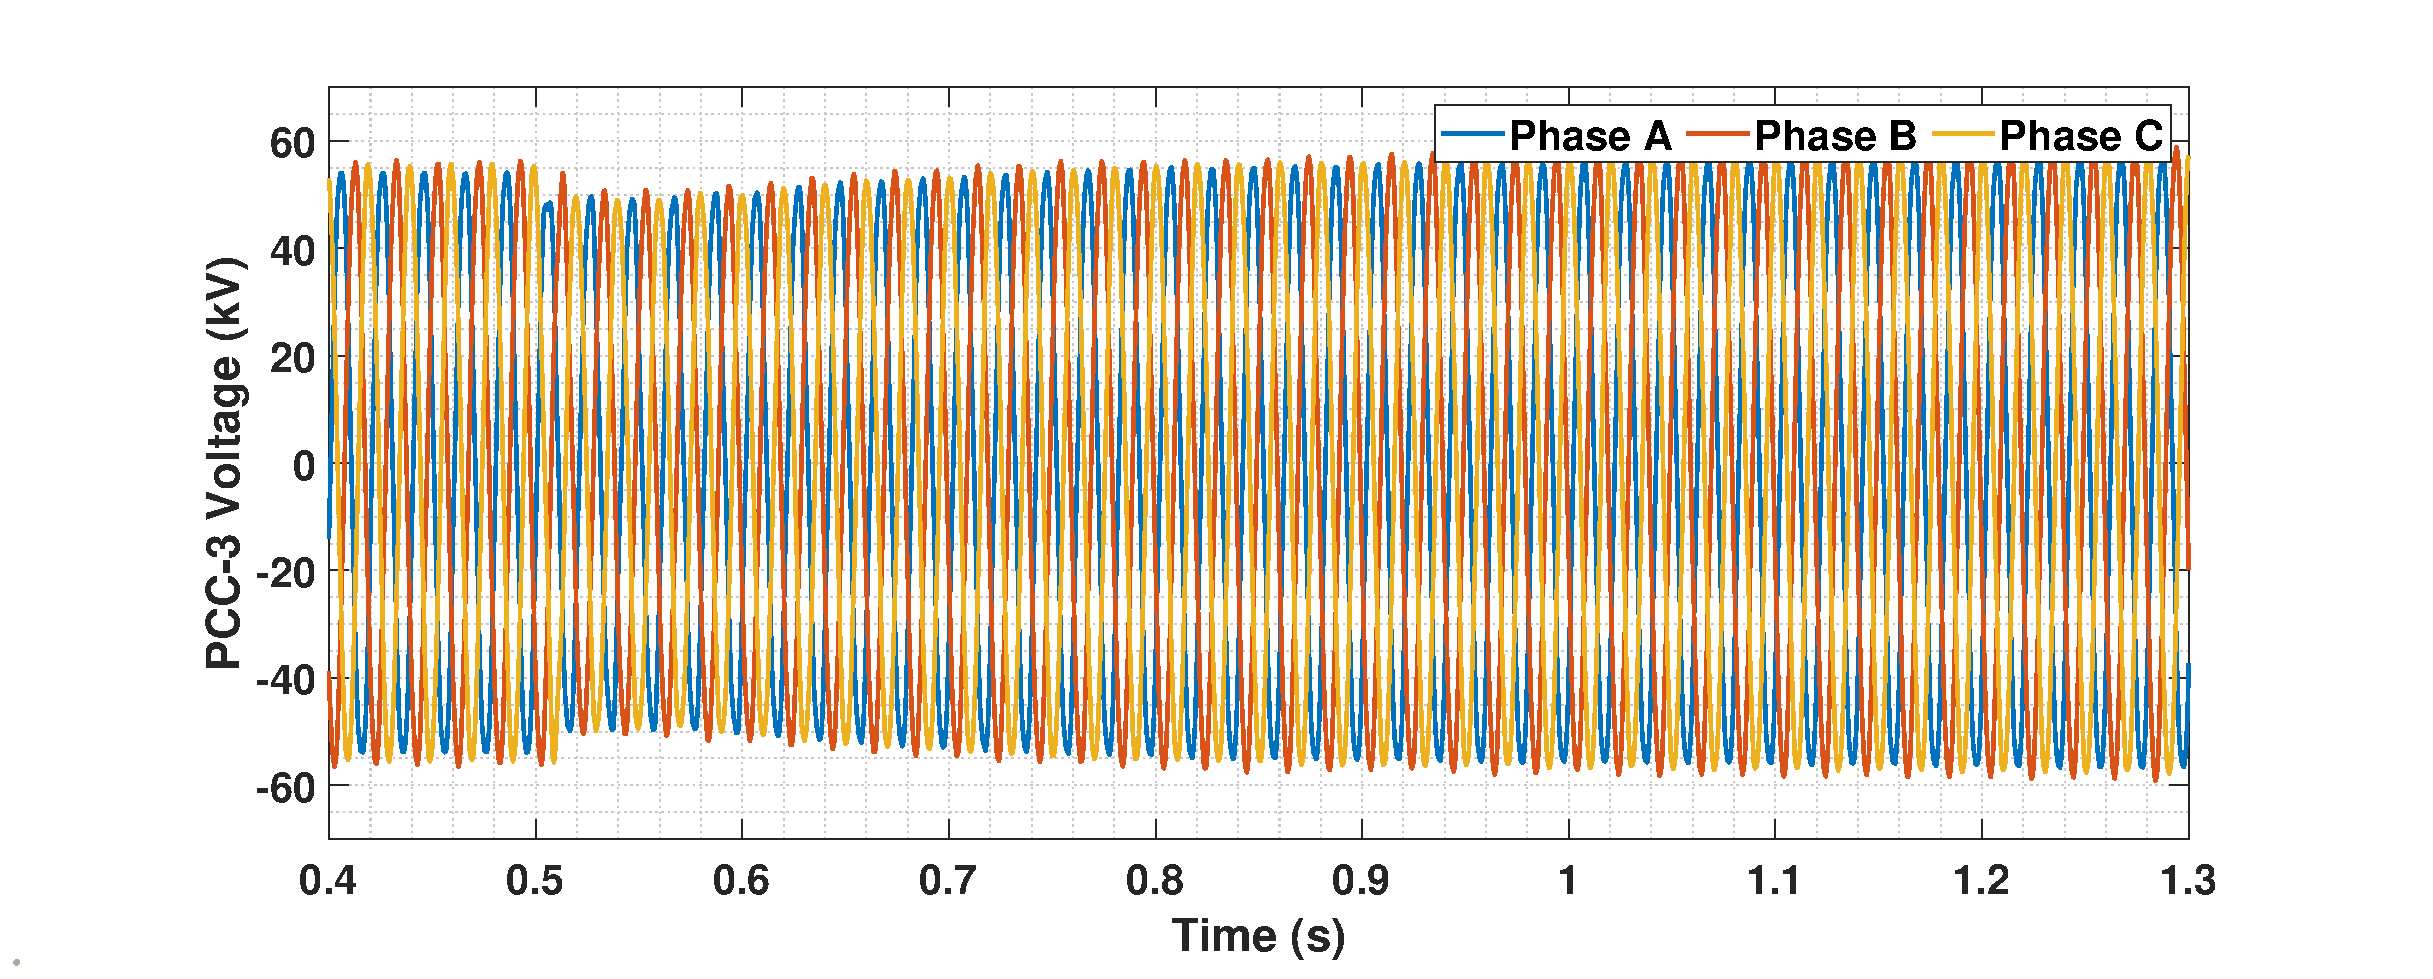
\includegraphics[height = 7cm,width = \textwidth]{Diagrams/Appendix_C/VABC_WT3_WT2off.eps}
    \caption{Voltages at PCC-3 upon OWF-2 disconnection event}
    \label{VABC_WT3_WT2off}
\end{figure}

\begin{figure}[H]
%\centering
%\hspace*{-1.2cm}
    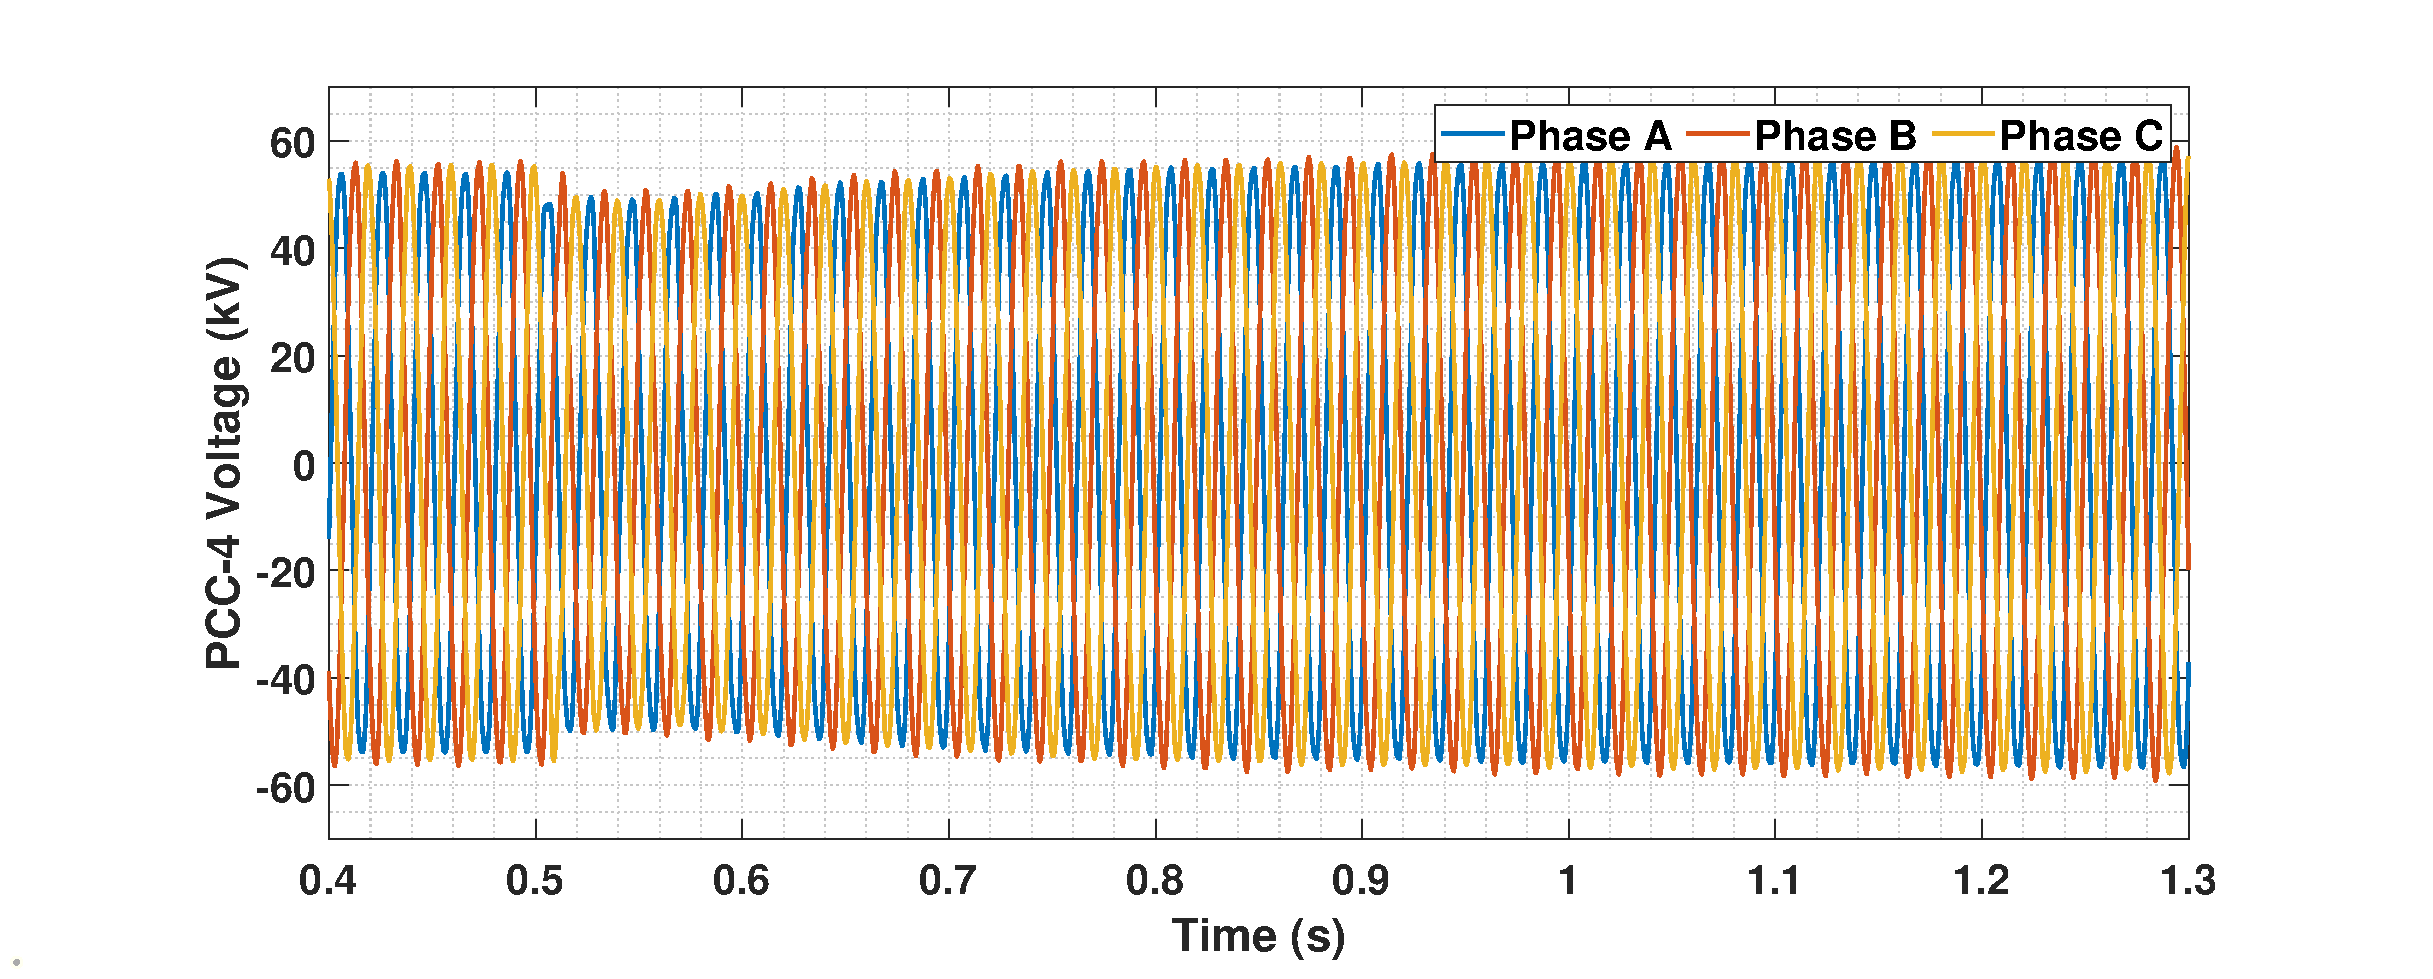
\includegraphics[height = 7cm,width = \textwidth]{Diagrams/Appendix_C/VABC_WT4_WT2off.eps}
    \caption{Voltages at PCC-4 upon OWF-2 disconnection event}
    \label{VABC_WT4_WT2off}
\end{figure}

\begin{figure}[H]
%\centering
%\hspace*{-1.2cm}
    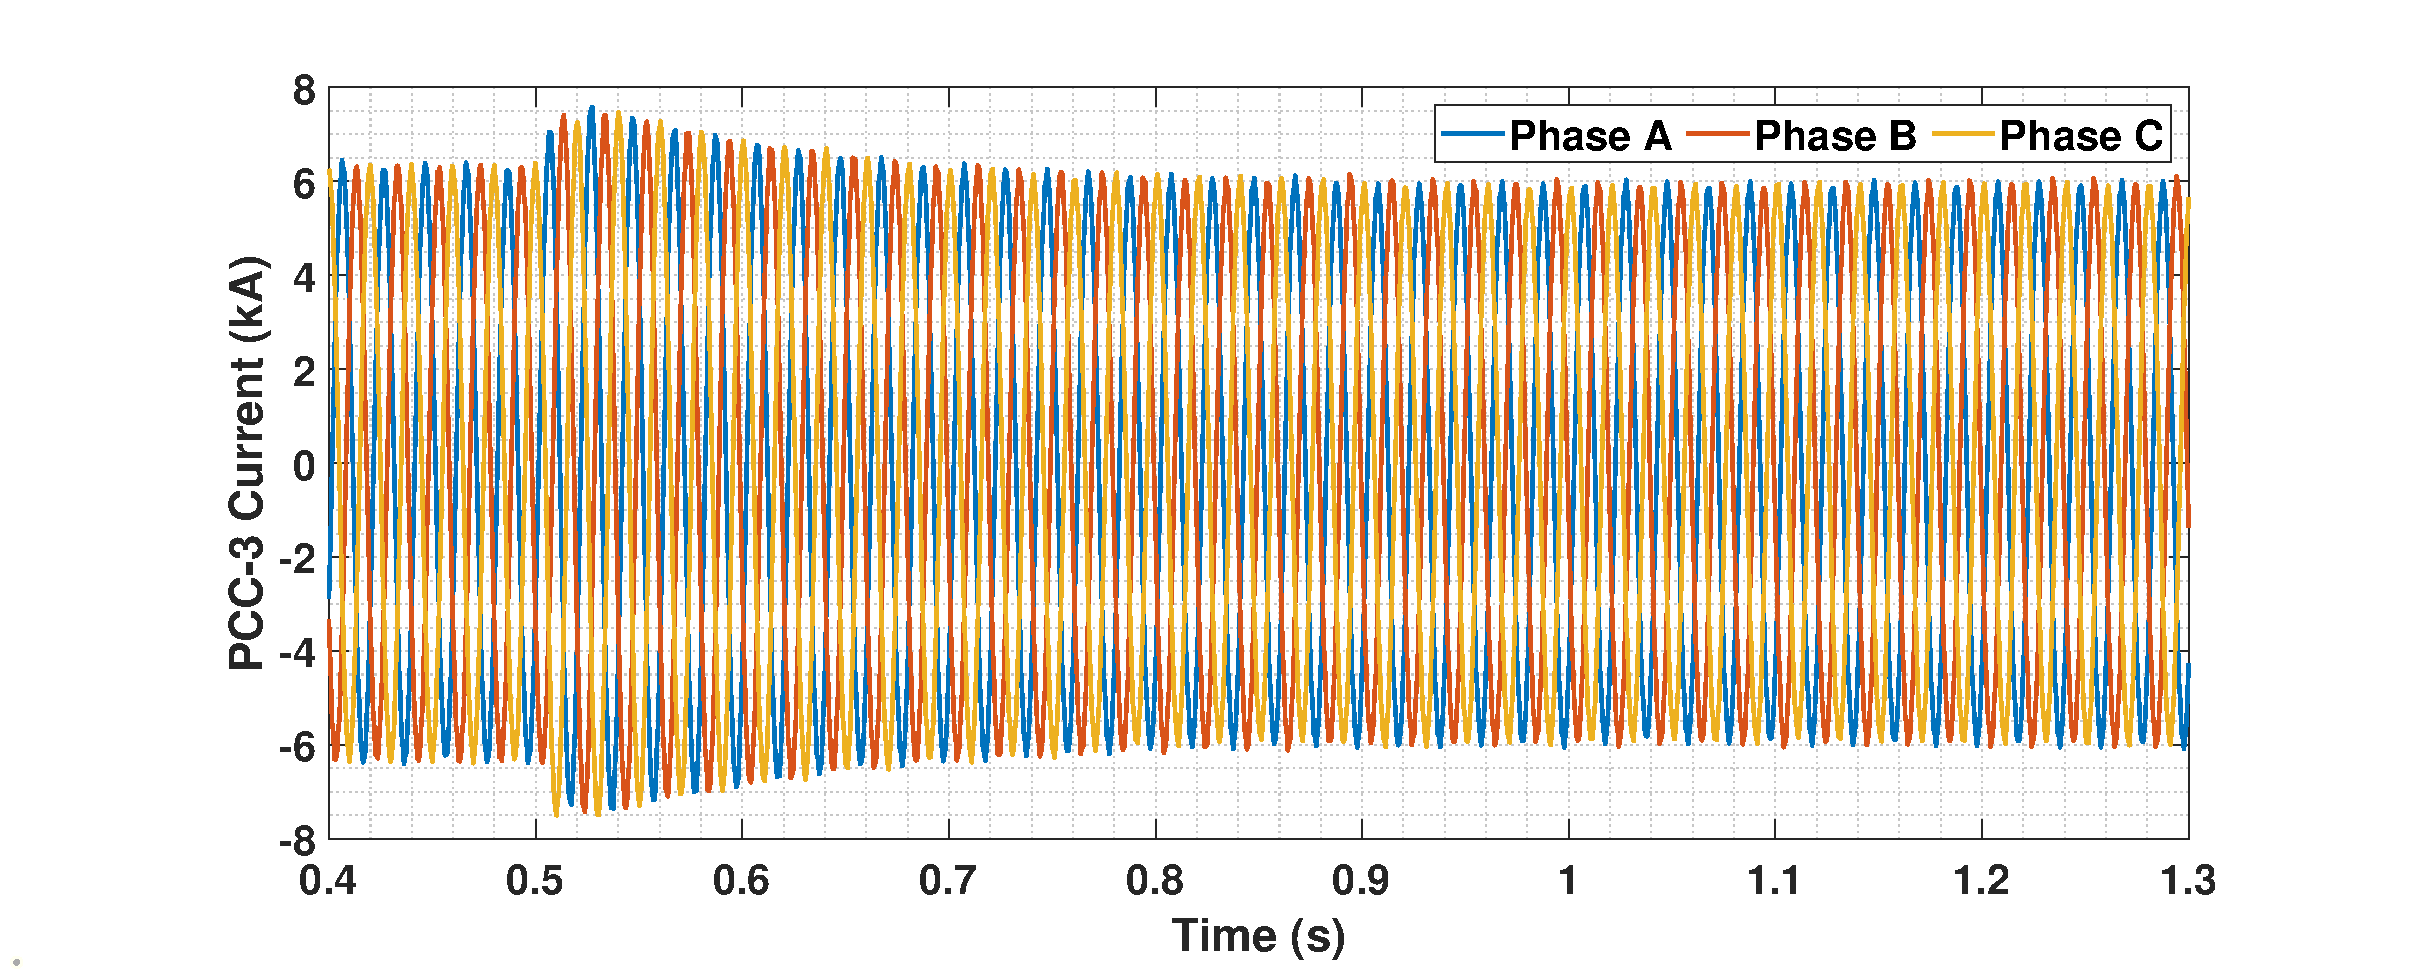
\includegraphics[height = 7cm,width = \textwidth]{Diagrams/Appendix_C/IABC_WT3_WT2off.eps}
    \caption{Currents in PCC-3 upon OWF-2 disconnection event}
    \label{IABC_WT3_WT2off}
\end{figure}

\begin{figure}[H]
%\centering
%\hspace*{-1.2cm}
    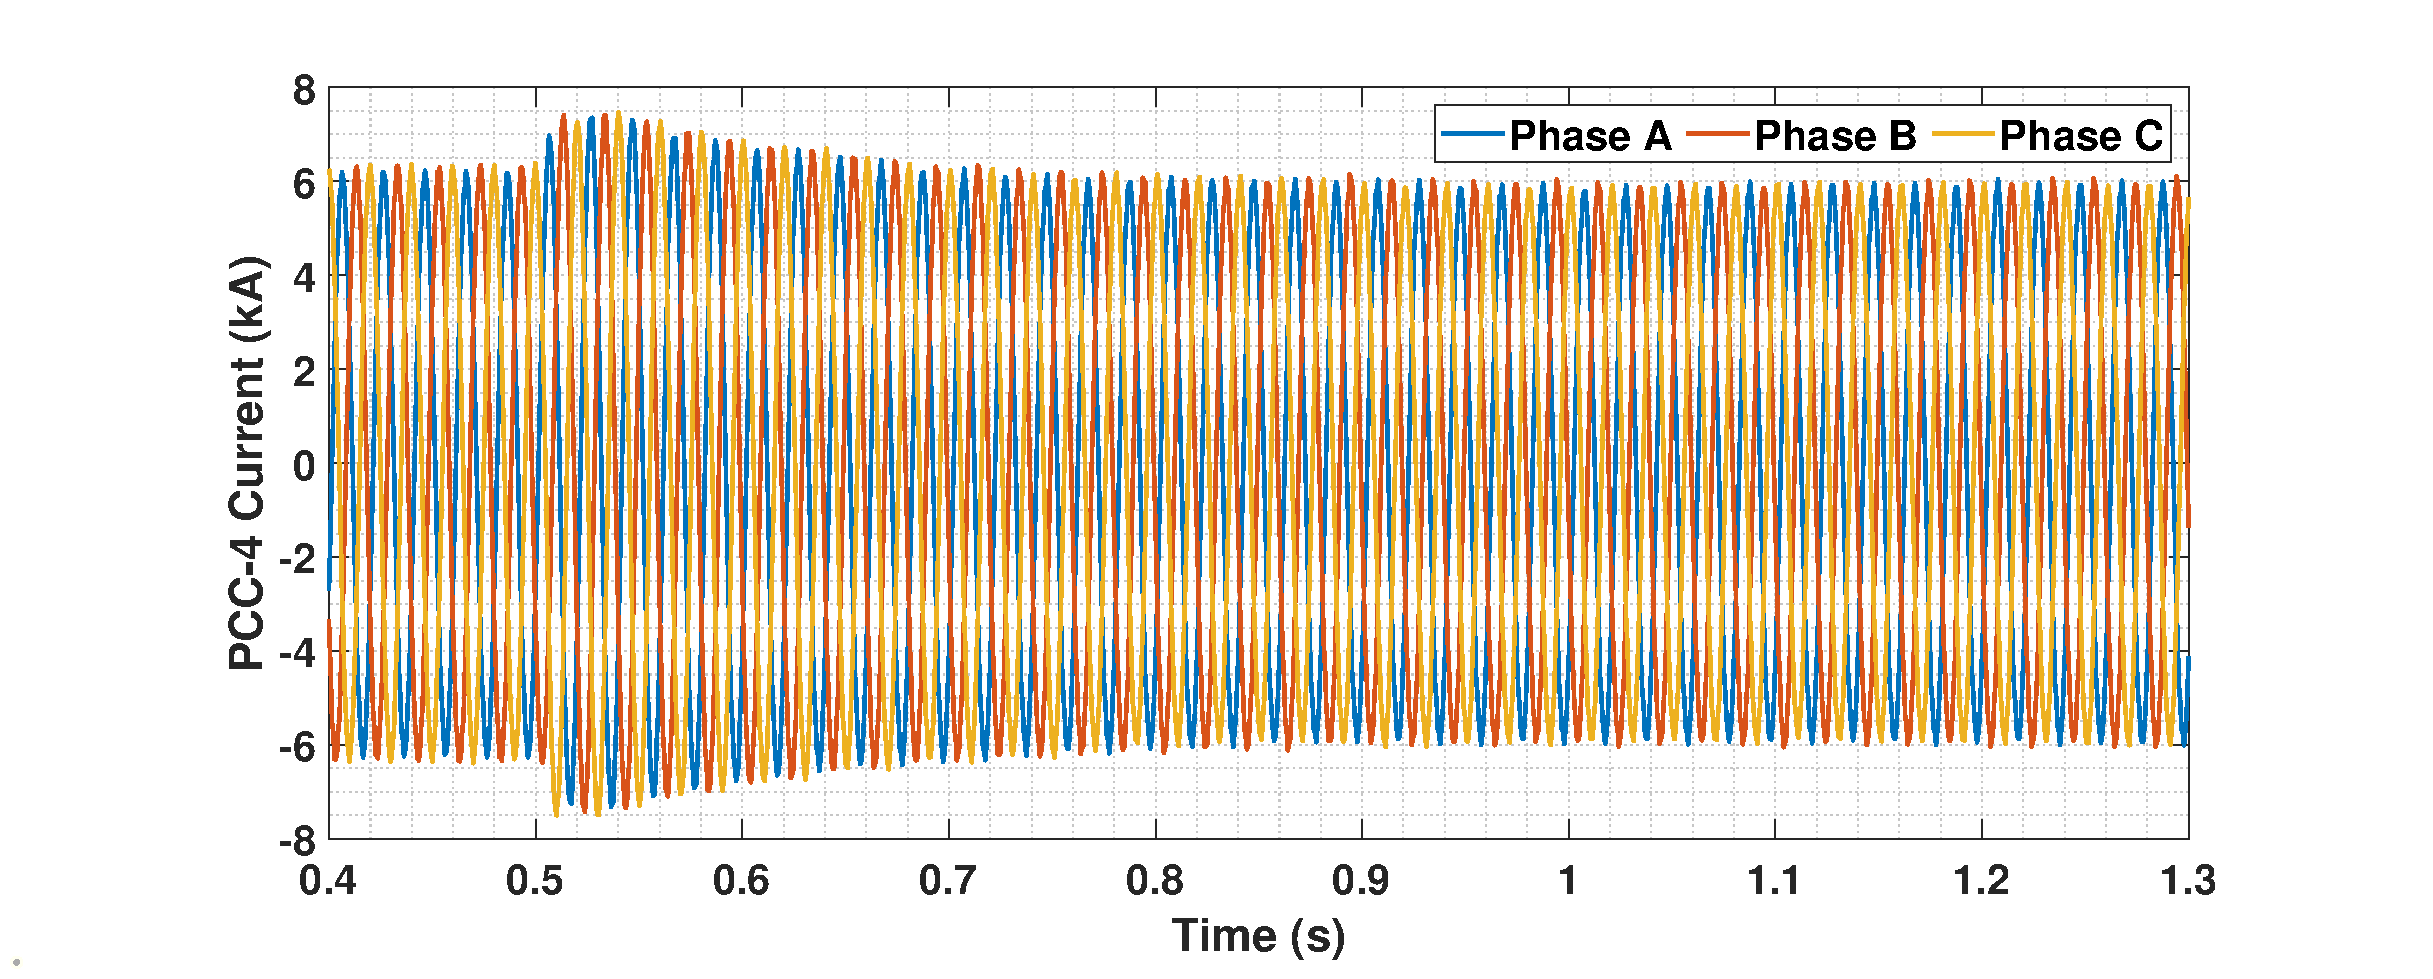
\includegraphics[height = 7cm,width = \textwidth]{Diagrams/Appendix_C/IABC_WT4_WT2off.eps}
    \caption{Currents in PCC-4 upon OWF-2 disconnection event}
    \label{IABC_WT4_WT2off}
\end{figure}

\subsection{Three-phase fault line to ground fault in the middle of cable-1}

\begin{figure}[H]
%\centering
%\hspace*{-1.2cm}
    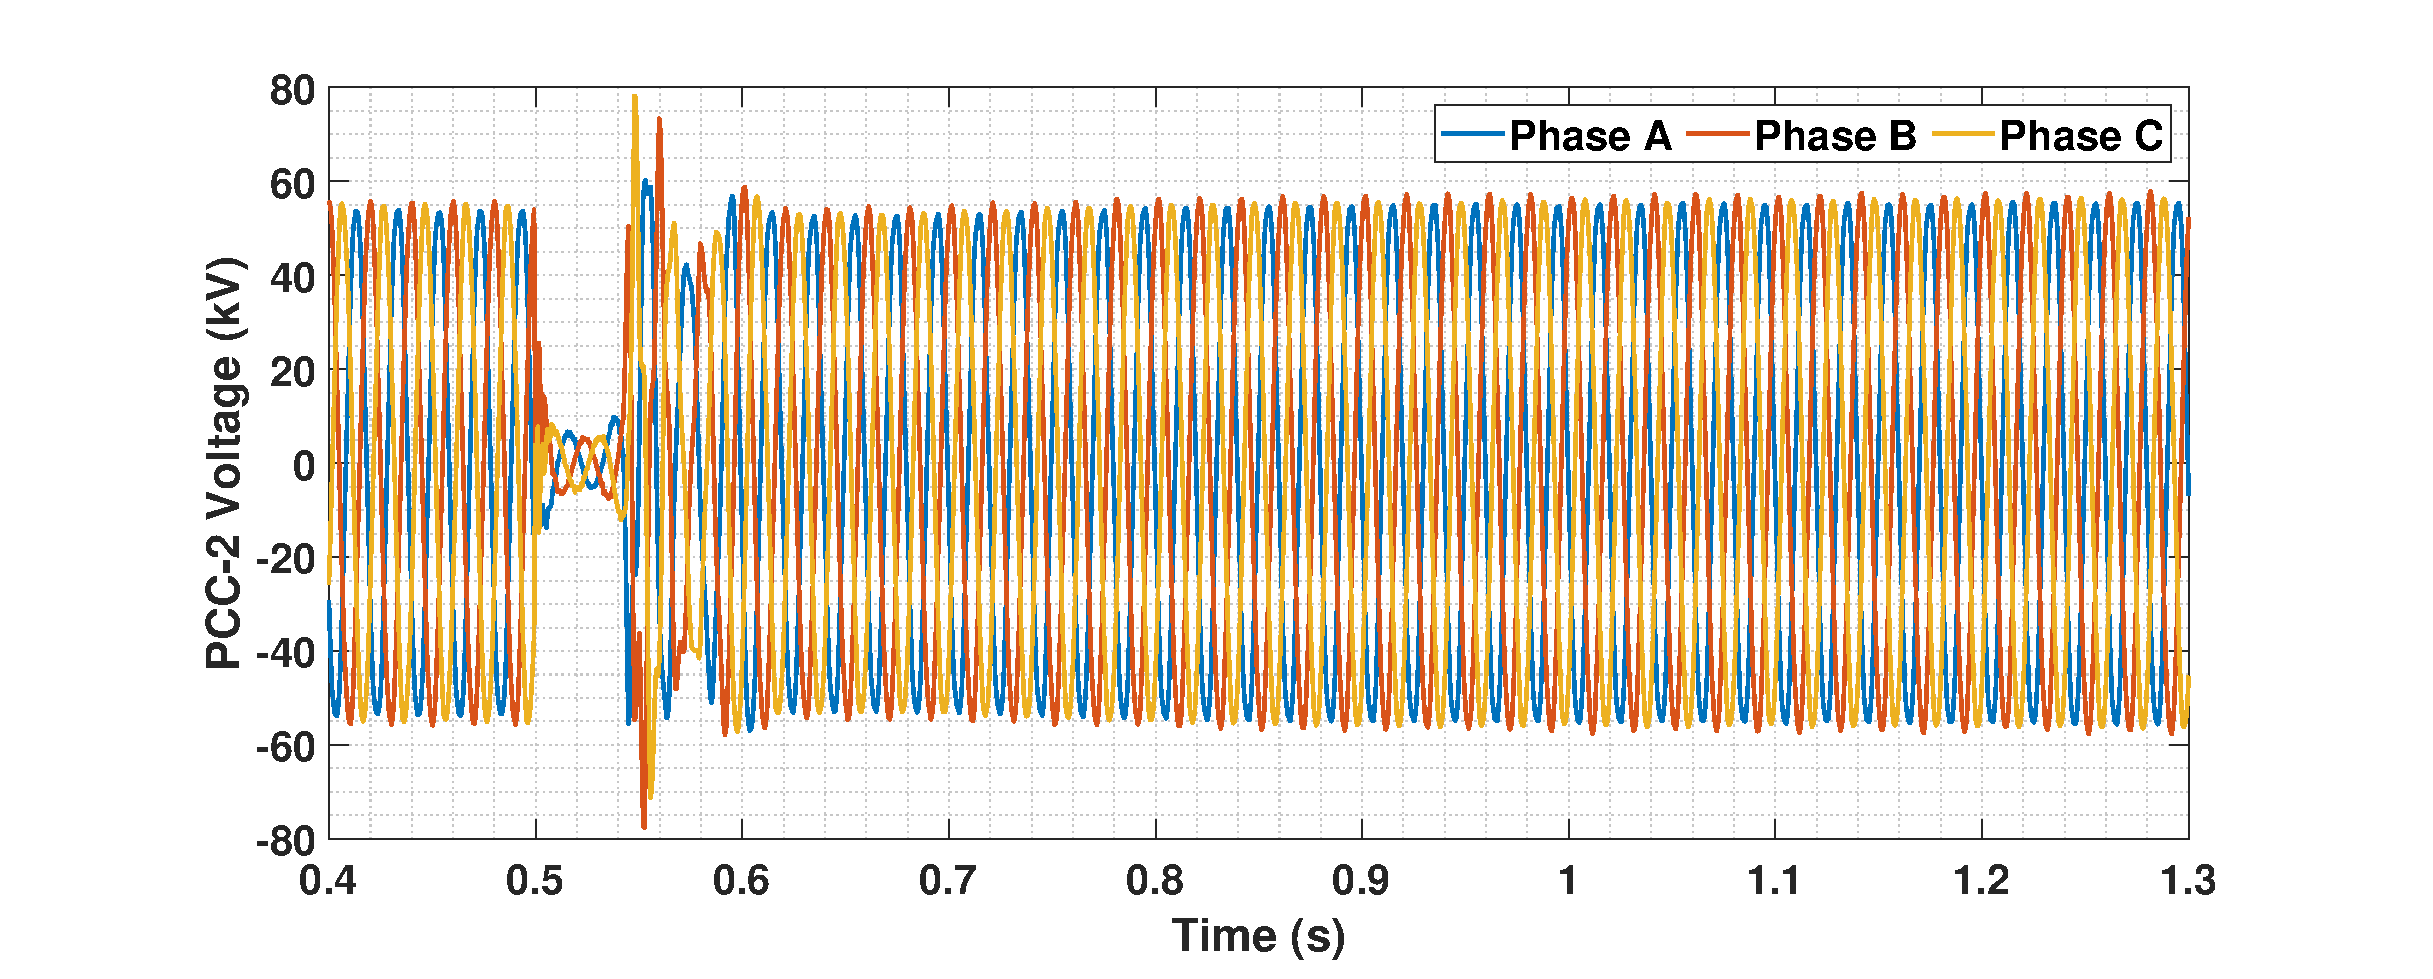
\includegraphics[height = 7cm,width = \textwidth]{Diagrams/Appendix_C/VABC_WT2_3phaseSC.eps}
    \caption{Voltages at PCC-2 upon three-phase line to ground fault in the middle of cable-1}
    \label{VABC_WT2_3phaseSC}
\end{figure}

\begin{figure}[H]
%\centering
%\hspace*{-1.2cm}
    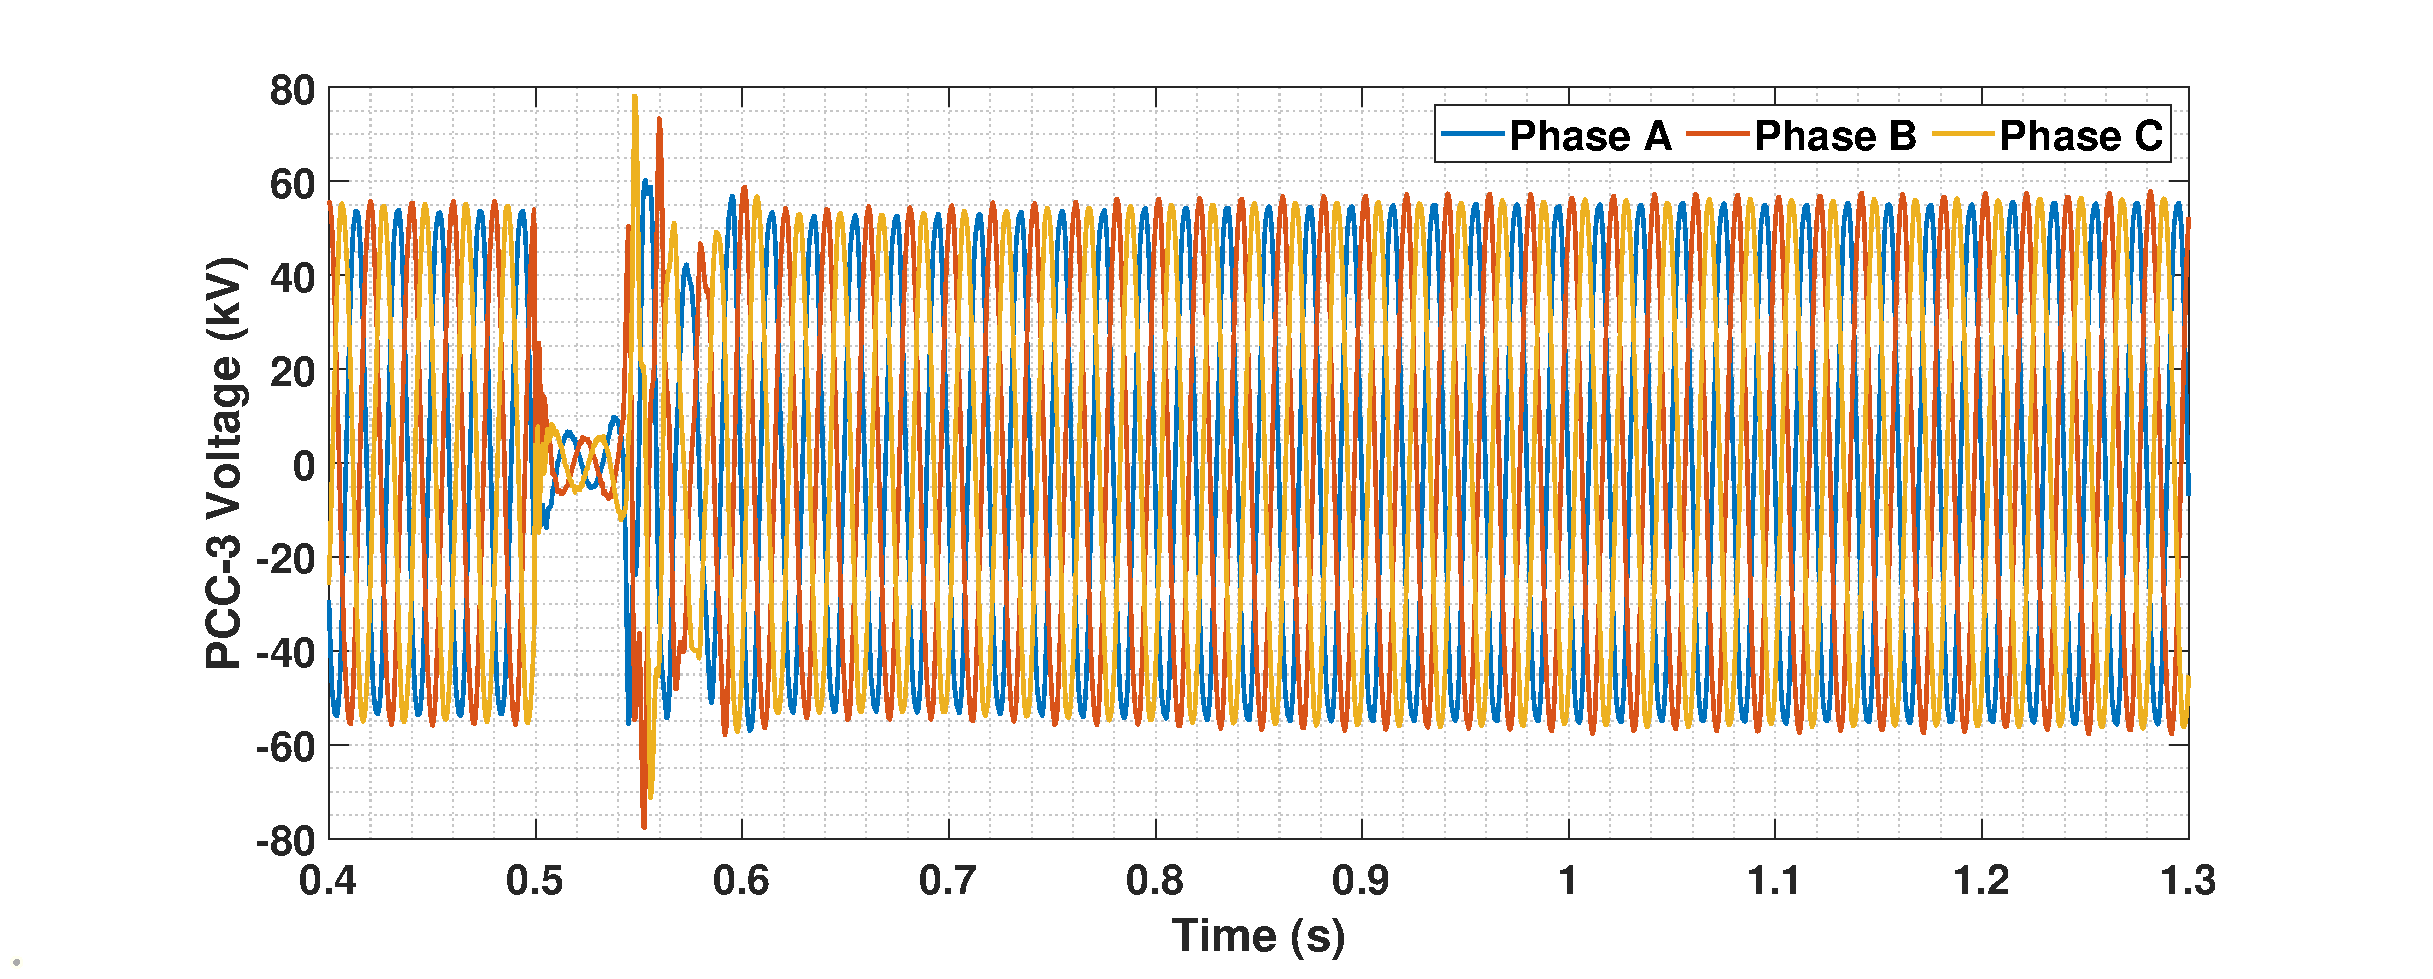
\includegraphics[height = 7cm,width = \textwidth]{Diagrams/Appendix_C/VABC_WT3_3phaseSC.eps}
    \caption{Voltages at PCC-3 upon three-phase line to ground fault in the middle of cable-1}
    \label{VABC_WT3_3phaseSC}
\end{figure}

\begin{figure}[H]
%\centering
%\hspace*{-1.2cm}
    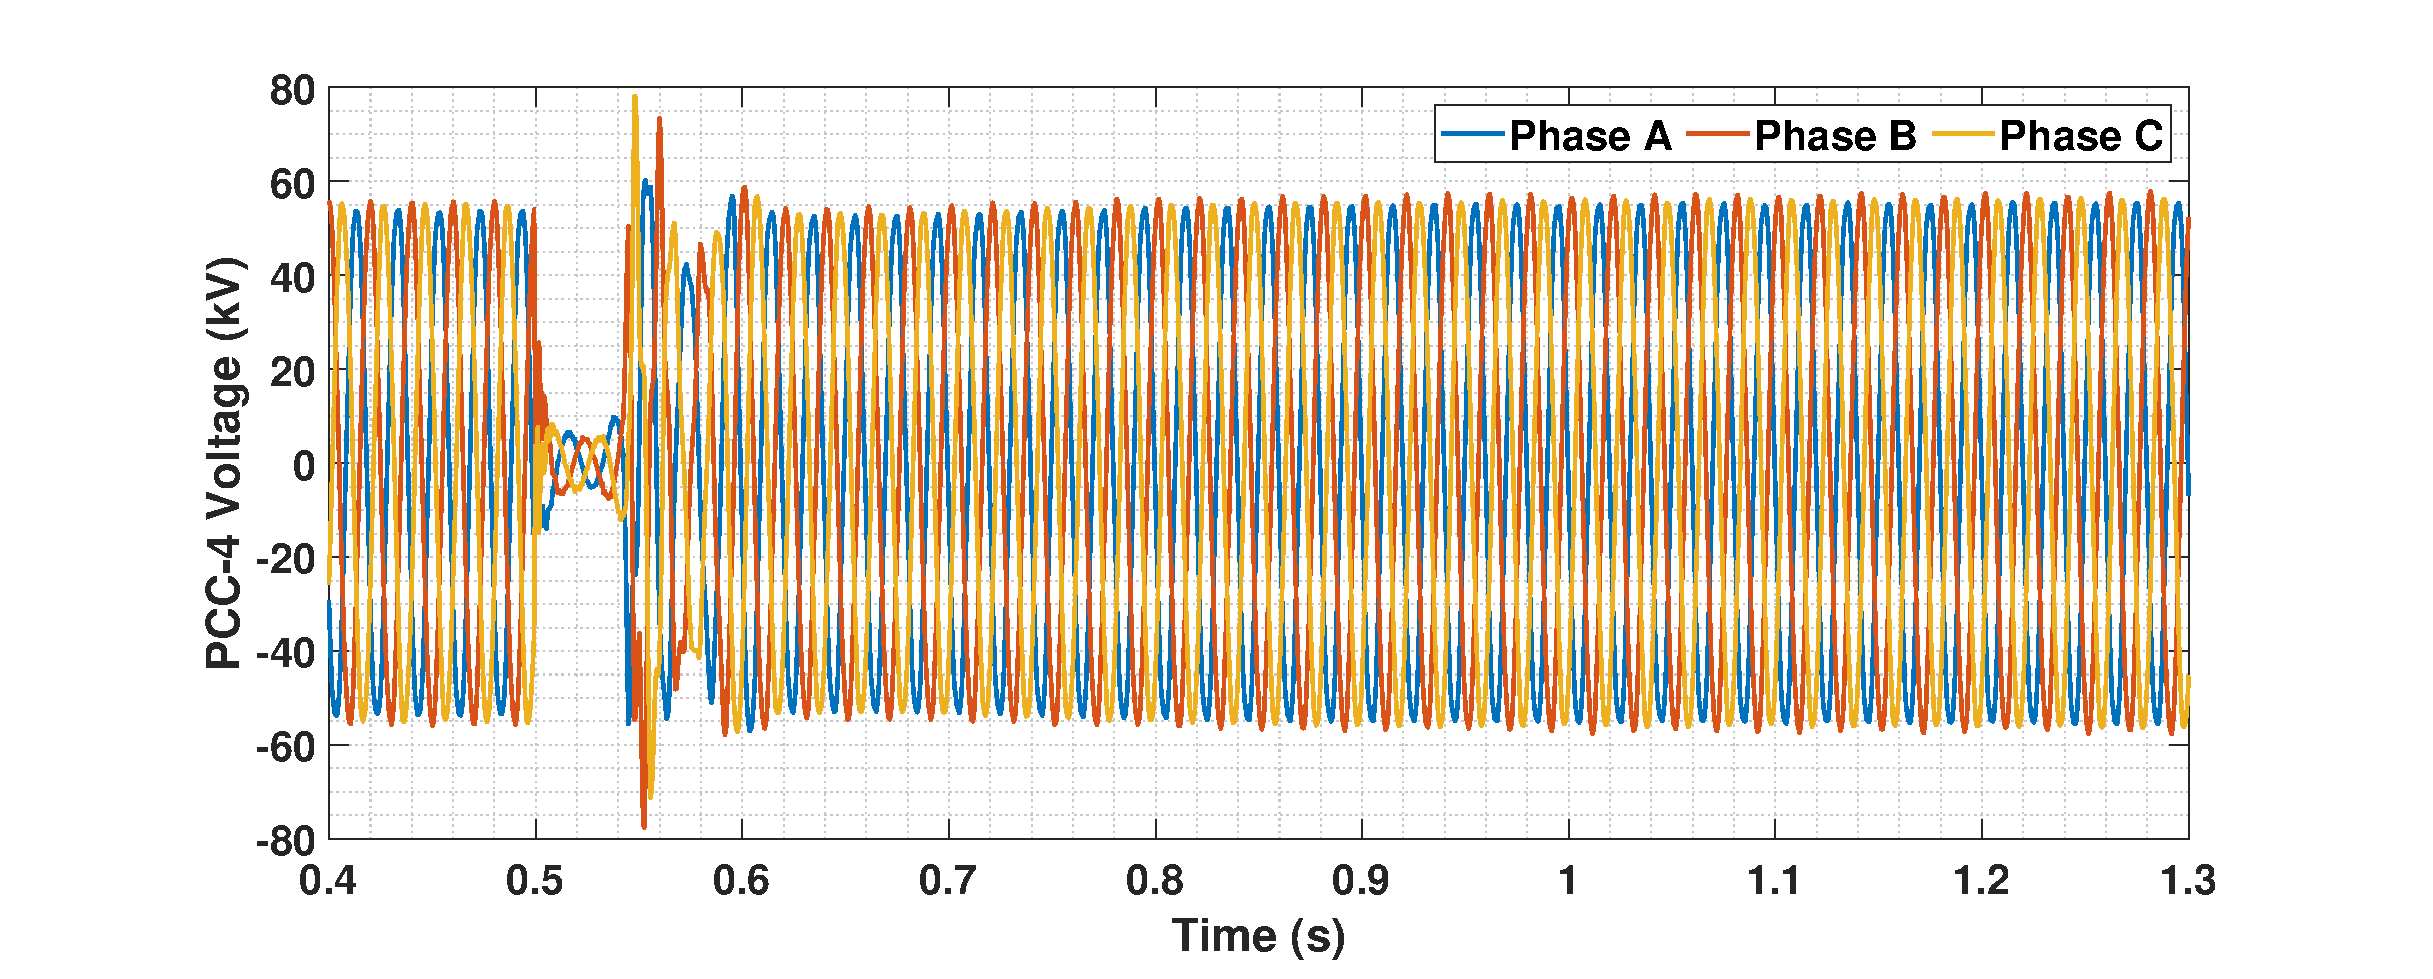
\includegraphics[height = 7cm,width = \textwidth]{Diagrams/Appendix_C/VABC_WT4_3phaseSC.eps}
    \caption{Voltages at PCC-4 upon three-phase line to ground fault in the middle of cable-1}
    \label{VABC_WT4_3phaseSC}
\end{figure}

\begin{figure}[H]
%\centering
%\hspace*{-1.2cm}
    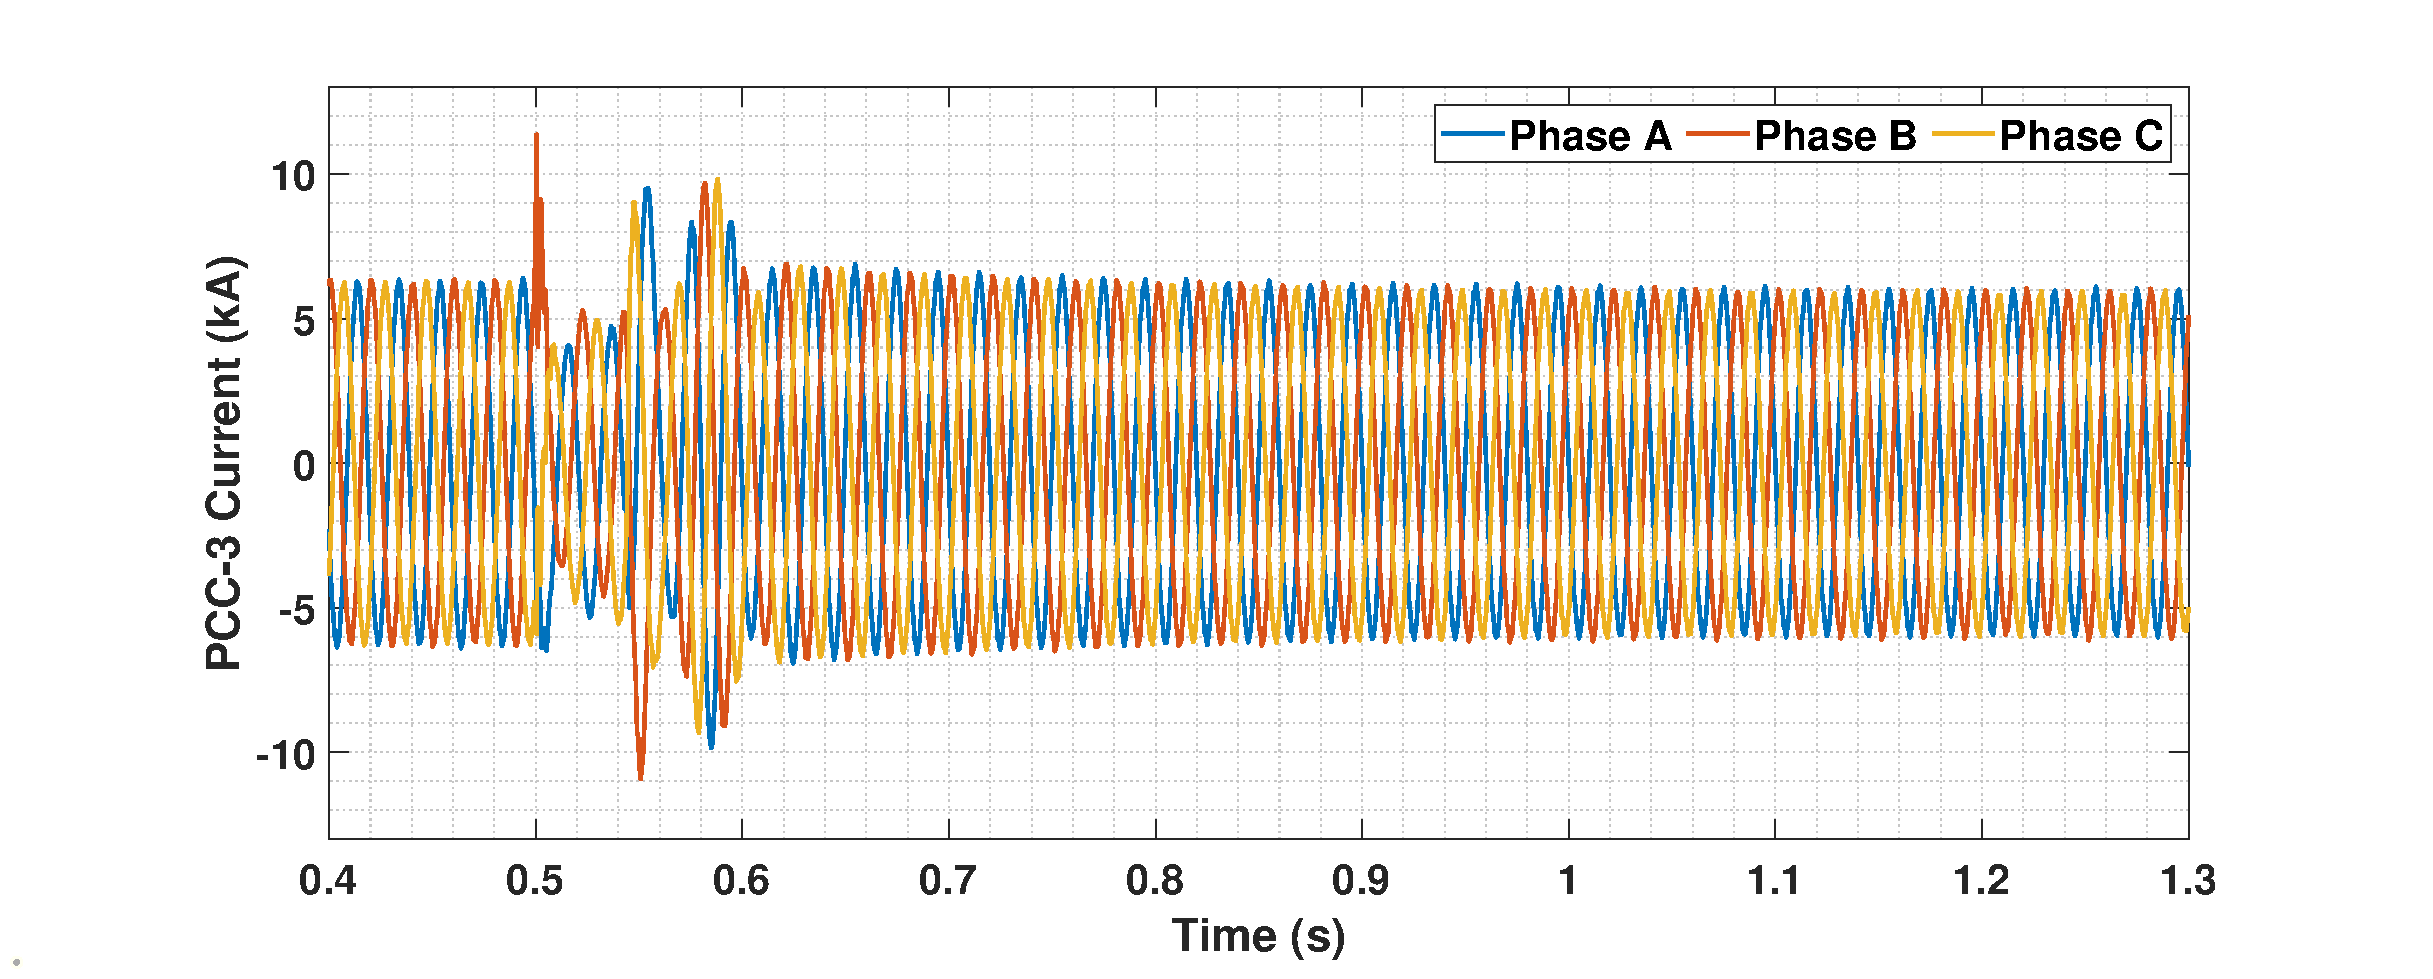
\includegraphics[height = 7cm,width = \textwidth]{Diagrams/Appendix_C/IABC_WT3_3phaseSC.eps}
    \caption{Currents in PCC-3 upon three-phase line to ground fault in the middle of cable-1}
    \label{IABC_WT3_3phaseSC}
\end{figure}

\begin{figure}[H]
%\centering
%\hspace*{-1.2cm}
    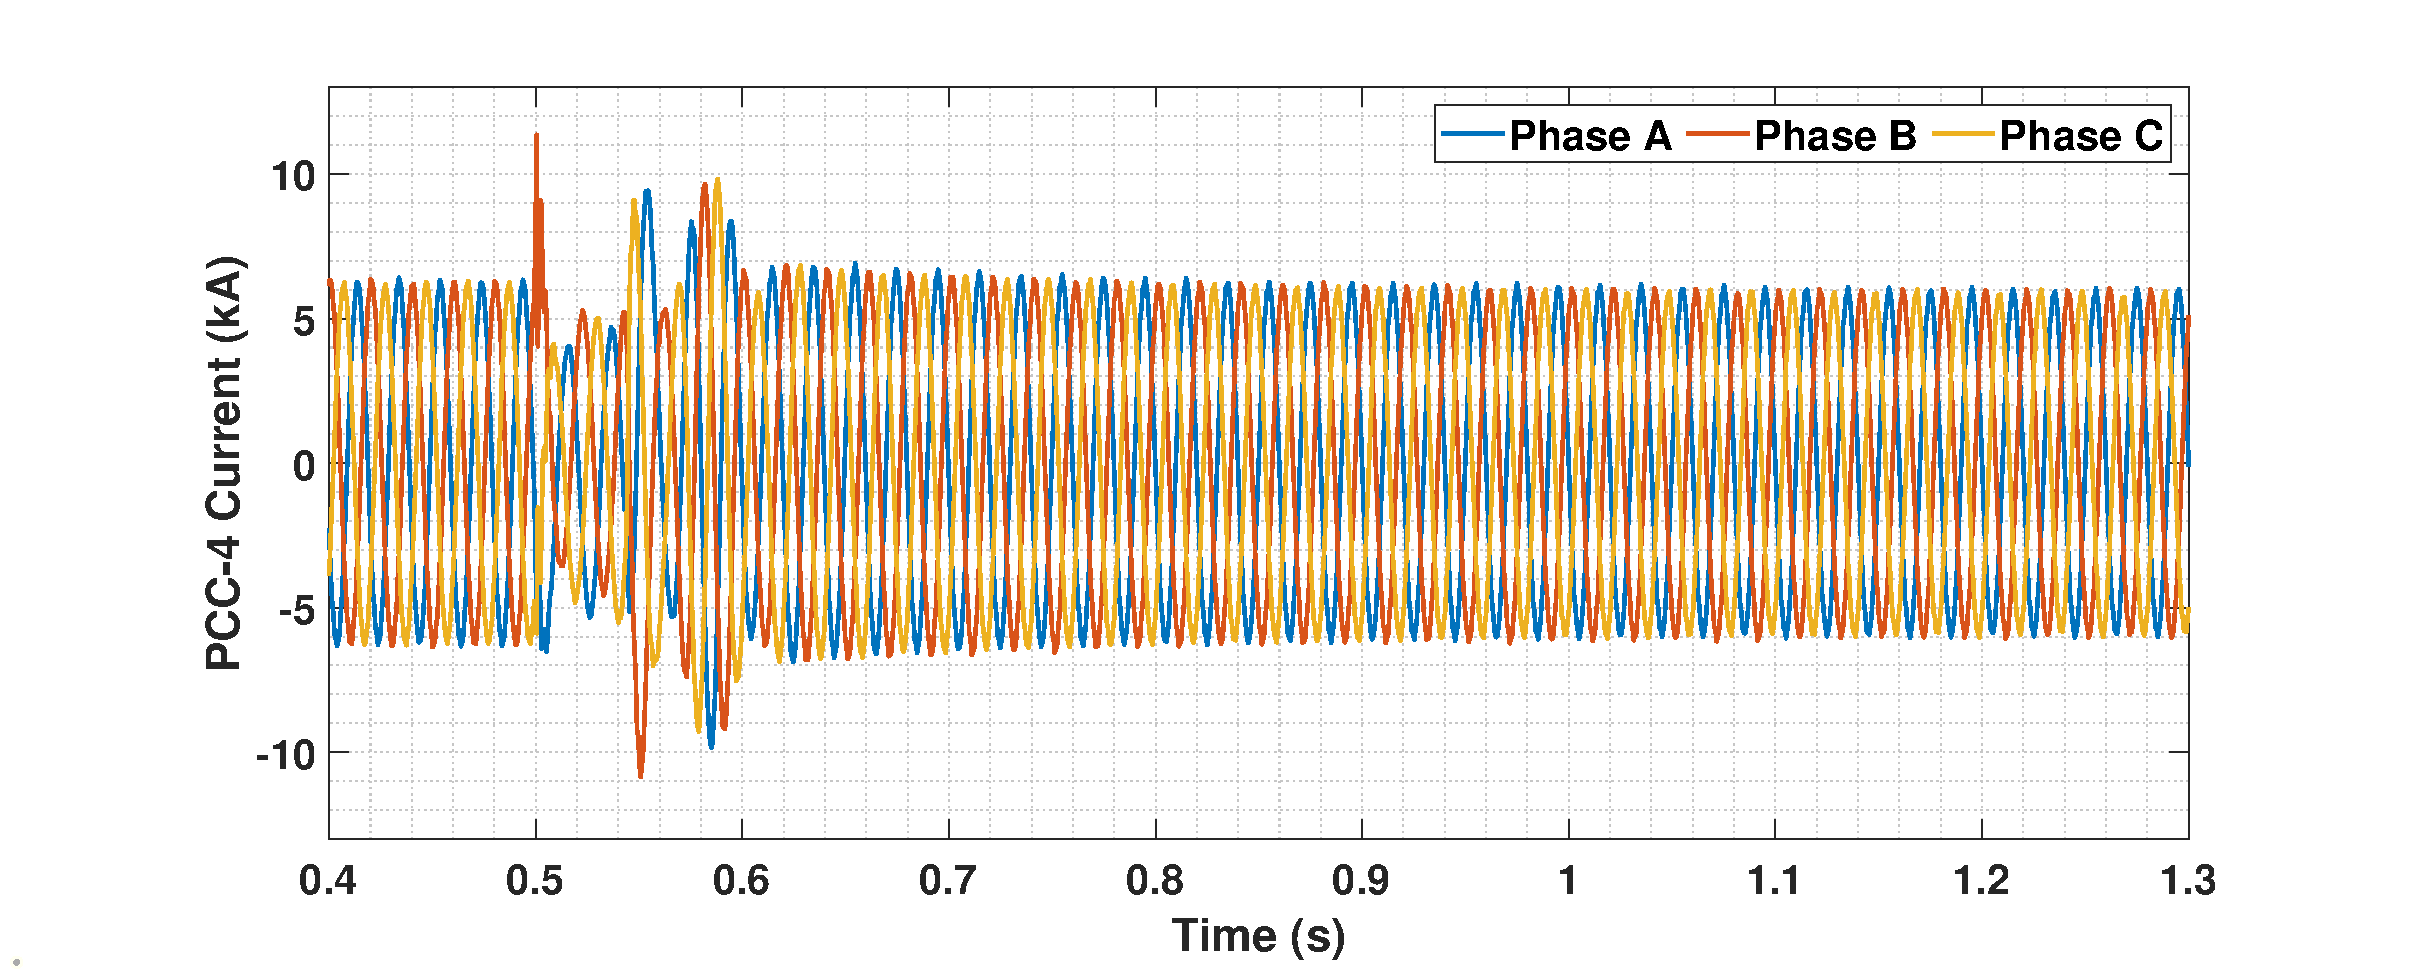
\includegraphics[height = 7cm,width = \textwidth]{Diagrams/Appendix_C/IABC_WT4_3phaseSC.eps}
    \caption{Currents in PCC-4 upon three-phase line to ground fault in the middle of cable-1}
    \label{IABC_WT4_3phaseSC}
\end{figure}

\begin{figure}[H]
%\centering
%\hspace*{-1.2cm}
    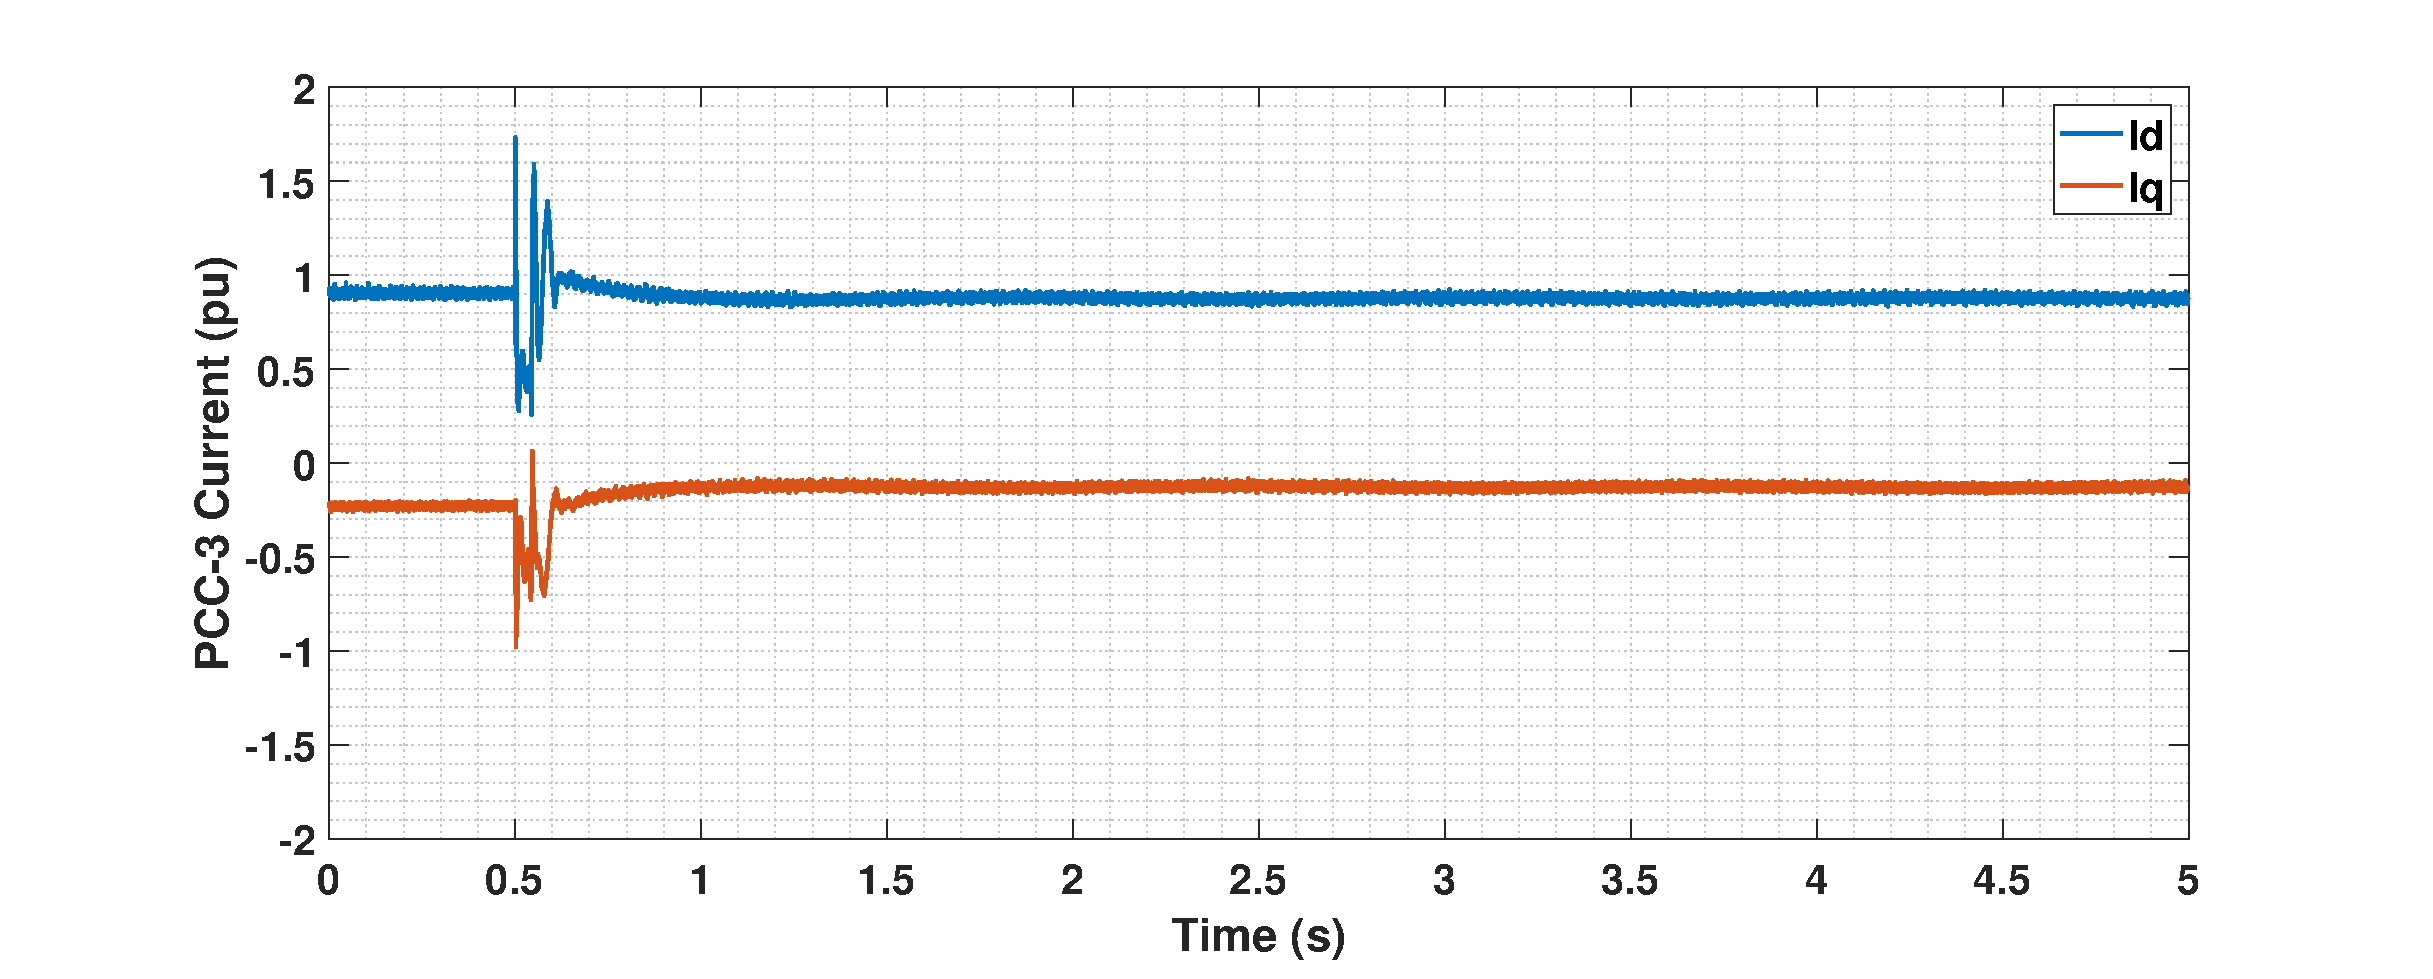
\includegraphics[height = 7cm,width = \textwidth]{Diagrams/Appendix_C/IDQ_WT3_3phaseSC.eps}
    \caption{Currents in d and q axes in PCC-3 upon three-phase line to ground fault in the middle of cable-1}
    \label{IDQ_WT3_3phaseSC}
\end{figure}

\begin{figure}[H]
%\centering
%\hspace*{-1.2cm}
    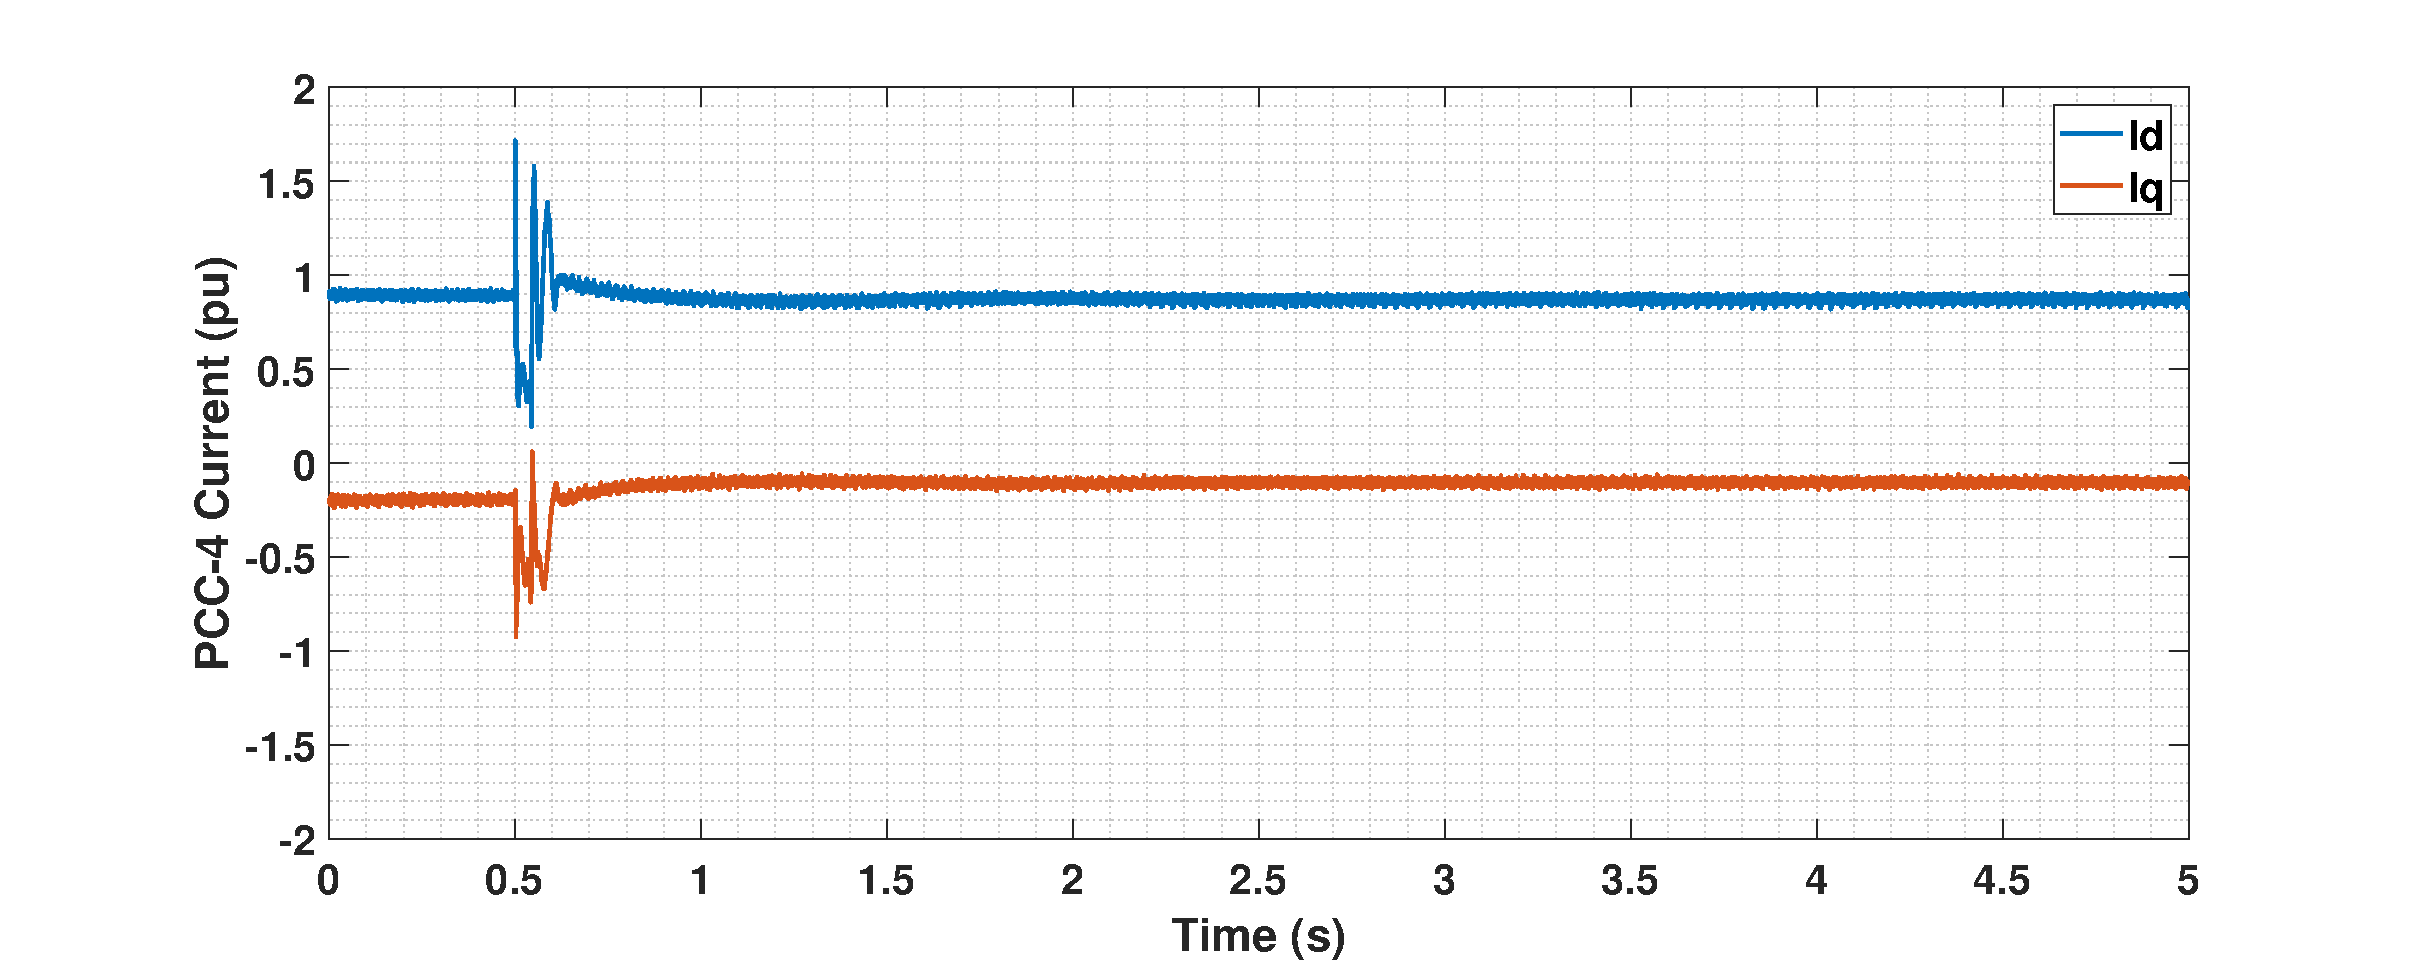
\includegraphics[height = 7cm,width = \textwidth]{Diagrams/Appendix_C/IDQ_WT4_3phaseSC.eps}
    \caption{Currents in d and q axes in PCC-4 upon three-phase line to ground fault in the middle of cable-1}
    \label{IDQ_WT4_3phaseSC}
\end{figure}